\documentclass{article}

% ==========================================================================
% chi-VLA, NeurIPS 2026 Neural Network Artifacts workshop submission
% Compile: pdflatex -interaction=nonstopmode chi-vla-neuralartifacts.tex  (twice)
% ==========================================================================

\PassOptionsToPackage{numbers,sort&compress}{natbib}
\usepackage[dblblindworkshop]{neurips_2026}
\workshoptitle{Neural Network Artifacts as a New Data Modality}
\usepackage[utf8]{inputenc}
\usepackage[T1]{fontenc}
\usepackage{amsmath,amssymb,amsfonts}
\usepackage{booktabs}
\usepackage{graphicx}
\usepackage{xcolor}
\usepackage{tikz}
\usetikzlibrary{positioning,fit,backgrounds,arrows.meta}
\usepackage[colorlinks=true,linkcolor=blue,citecolor=blue,urlcolor=blue]{hyperref}
\usepackage{url}
\usepackage{float}
\usepackage{microtype}
\newcommand{\chivla}{$\chi$-VLA}
\newcommand{\R}{\mathbb{R}}

\title{\textbf{A Robot Policy Designed as a Weight-Space Artifact}\\[0.15em]
\textbf{Exact Tensor Structure in a Capable VLA}\\[0.35em]
\large Rational conversion, reduced-Gram analysis, and causal intervention}
\author{}
\date{}

\begin{document}
\maketitle

\begin{abstract}
Can model weights be made a first-class analysis artifact without sacrificing closed-loop
capability? We introduce \chivla, a $20.1$M-parameter vision-language-action policy whose
learned map contains only bilinear, linear, and rational operations. Its checkpoint therefore
specifies an explicit rational tensor program. A mechanical audit finds no softmax, standard
activation, or ordinary normalization, and local reconstructions agree with deployment near
the float32 precision floor. We derive an exact weight-based decomposition of each
softmax-free attention layer, including rational query-key normalization, and reduce its
otherwise intractable coefficient Gram to $O(d^2)$ storage. In the primary screen, all $36$
trained block-head pairs favor the rank-$128$ weight-derived subspace over fixed equal-rank
random controls. The full eight-block appendix screen finds the effect in $83/96$ pairs and
reveals depth-specific negative controls. At the policy's visual bond, a causally ranked
$64$-dimensional subspace preserves $18/20$ closed-loop successes, while a random subspace
preserves none. The artifact is behaviorally nontrivial: the policy reaches
$93.7\%\pm0.8\%$ on LIBERO-Object over three seeds. The first direct coefficient-edit screen,
however, fails its preregistered selectivity gate. We therefore present a capable model
artifact with exact layerwise structure and a causal analysis surface, not yet a semantic or
selectively editable weight-space interface.
\end{abstract}

% ============================================================================
\section{Introduction}
% ============================================================================

Neural checkpoints are usually treated as opaque containers for functions. Their weights can
still support post-hoc analysis, but softmax, ordinary activations, and input-dependent
normalization obstruct direct conversion of the complete learned map into an explicit
polynomial or rational tensor object. Bilinear language and vision models show that changing
the primitives can expose useful weight structure \cite{pearce,chinets}. Whether such a model
artifact can remain behaviorally competitive in continuous closed-loop control is unresolved.

We study two linked questions:

\begin{quote}
\emph{Can the learned weights of a specialist VLA specify an explicit rational tensor program,
and can that artifact expose exact structure with a measurable causal consequence?}
\end{quote}

Our contributions are:

\begin{enumerate}
  \item We construct and mechanically certify a complete VLA from tensor-compatible primitives.
        A rational normalization supplies input-specific scaling without leaving the rational
        function class.
  \item We derive exact weight-based structure through each softmax-free attention layer and an
        $O(d^2)$ reduced-Gram calculation that avoids materializing its high-order coefficient
        tensor.
  \item We test the artifact at behavioral scale. Exact subspaces beat fixed random controls,
        and a causally ranked visual subspace preserves $18/20$ closed-loop successes while a
        random subspace preserves none.
  \item We establish that the analyzed artifact is a capable policy, reaching
        $93.7\%\pm0.8\%$ over three LIBERO-Object seeds, while reporting a language shortcut and
        a failed coefficient-surgery gate that bound the current interpretation.
\end{enumerate}

This paper does not claim current state of the art. It also does not claim that comparable
mechanisms are impossible to obtain from conventional policies. The empirical question is
whether the algebraic policy makes them more direct, stable, and selectively editable than
matched post-hoc methods.

% ============================================================================
\section{A rational tensor robot policy}
\label{sec:model}
% ============================================================================

\subsection{Tensor-compatible primitives}

\paragraph{Homogeneous coordinate.}
We write $\bar x=[1;x]$. The constant coordinate allows a multiplicative layer to represent
bias, linear, and quadratic terms in one contraction.

\paragraph{Bilinear feed-forward block.}
For $L,R\in\R^{r\times(d+1)}$ and $D\in\R^{d\times r}$,
\begin{equation}
\mathrm{BFFN}(x)
=D\left[(L\bar x)\odot(R\bar x)\right],
\qquad
y_o=\sum_{i,j}\left(\sum_{\rho}D_{o\rho}L_{\rho i}R_{\rho j}\right)\bar x_i\bar x_j .
\label{eq:bffn}
\end{equation}
The three matrices are a CP factorization of the order-three coefficient tensor.

\paragraph{Softmax-free bilinear attention.}
Each head forms two query-key systems and one value stream:
\begin{equation}
Y=C\left[M\odot(Q_1K_1^\top)\odot(Q_2K_2^\top)/s\right]V .
\label{eq:attention}
\end{equation}
Here $M$ is a fixed causal mask, $C$ is fixed row scaling, and $s$ is fixed. All learned
query, key, value, and output maps are linear. Equation~\ref{eq:attention} is therefore a
polynomial in its input activations.

\paragraph{Rational per-instance normalization.}
RMS normalization contains an input-dependent square root. We instead deploy a fixed rational
approximation $r(z)=P(z)/Q(z)$ to $1/\sqrt{z+\epsilon}$:
\begin{equation}
\mathrm{RNorm}(x)=x\,r\!\left(\frac{1}{d}\sum_{j=1}^{d}x_j^2\right).
\label{eq:rnorm}
\end{equation}
The deployed function is exactly rational. Projective coordinates carry each activation as a
pair $(N,D)$ representing $N/D$. Linear, bilinear, residual, and normalization operations
update the numerator and denominator without introducing a non-rational learned operation.

\begin{figure}[H]
\centering
\resizebox{0.96\textwidth}{!}{%
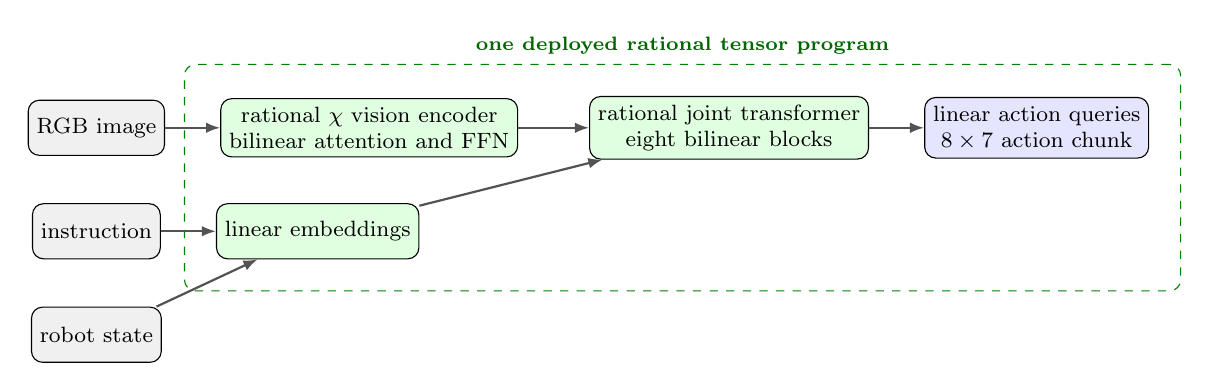
\begin{tikzpicture}[
  font=\footnotesize,
  box/.style={draw,rounded corners,align=center,minimum height=7mm,inner sep=3pt},
  inp/.style={box,fill=gray!12},
  prim/.style={box,fill=green!12},
  output/.style={box,fill=blue!10},
  arr/.style={-{Latex[length=1.8mm]},thick,gray!65!black},
  node distance=6mm and 7mm,
]
\node[inp] (img) {RGB image};
\node[inp, below=of img] (txt) {instruction};
\node[inp, below=of txt] (state) {robot state};
\node[prim, right=of img] (vision) {rational $\chi$ vision encoder\\bilinear attention and FFN};
\node[prim, right=of txt] (embed) {linear embeddings};
\node[prim, right=9mm of vision, minimum width=34mm] (joint) {rational joint transformer\\eight bilinear blocks};
\node[output, right=of joint] (action) {linear action queries\\$8\times7$ action chunk};
\draw[arr] (img) -- (vision);
\draw[arr] (txt) -- (embed);
\draw[arr] (state) -- (embed);
\draw[arr] (vision) -- (joint);
\draw[arr] (embed) -- (joint);
\draw[arr] (joint) -- (action);
\begin{scope}[on background layer]
\node[draw=green!50!black,dashed,rounded corners,fit=(vision)(embed)(joint)(action),
      inner sep=4mm,label={[green!40!black,font=\scriptsize\bfseries]above:one deployed rational tensor program}] {};
\end{scope}
\end{tikzpicture}}
\caption{\textbf{Deployed \chivla\ map.} The strongest checkpoints use one vision stream and a
linear continuous-action head. Every learned component inside the dashed boundary is linear,
bilinear, or rational.}
\label{fig:architecture}
\end{figure}

\subsection{Architecture and training}

The policy follows the high-level VLA sequence of visual encoding, language and state
embedding, joint processing, and action decoding \cite{openvla}. It uses a $64\times64$
agent-view image, an eight-dimensional robot state, a 26-token task vocabulary, and eight
action-query tokens. The joint backbone has width $384$, eight blocks, and twelve heads.
The action head maps each action-query state directly to seven continuous action dimensions.
The complete model has $20{,}137{,}352$ learned parameters.

Training uses $66{,}984$ demonstration frames, $40{,}000$ AdamW updates, batch size $256$,
cosine decay, bfloat16 arithmetic, and an exponential moving average. Closed-loop evaluation
uses a $180^\circ$ camera rotation to match the demonstration convention, canonical LIBERO
initial states, and fail-loud checks that verify every requested state was loaded.

\subsection{Mechanical certificate on the trained checkpoint}

Architecture definitions can differ from deployed code. We therefore audit the real
$189/200$ checkpoint at runtime and reconstruct representative operations from saved weights.

\begin{figure}[H]
\centering
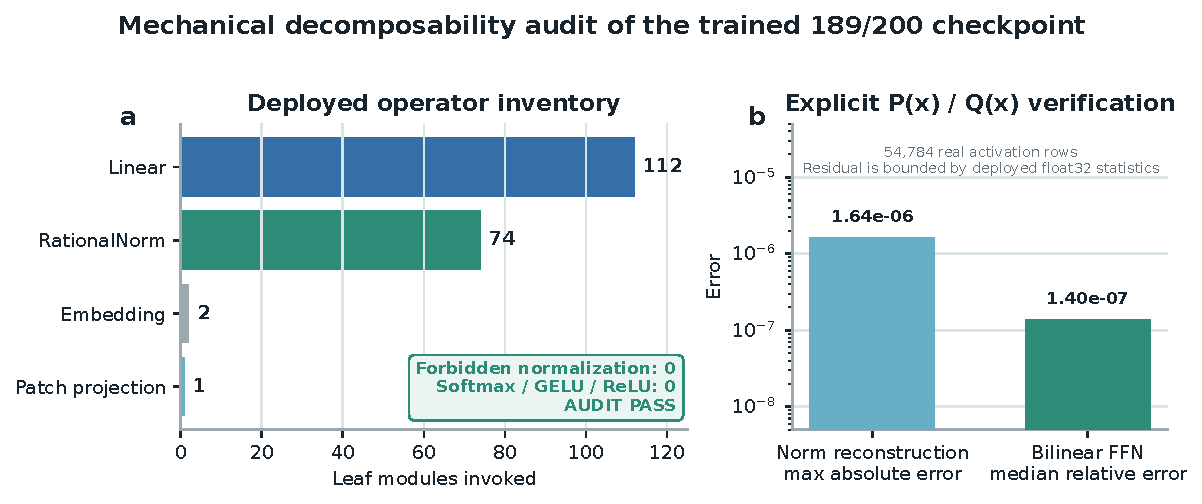
\includegraphics[width=0.88\textwidth]{../paper_figures/appendix_decomposability_audit.pdf}
\caption{\textbf{Mechanical audit of the trained rational checkpoint.} The runtime path invokes
$112$ linear maps, $74$ rational normalizers, two embeddings, and one linear patch projection.
No softmax, standard activation, or ordinary normalization is present. Reconstruction errors
are measured over $54{,}784$ real activation rows.}
\label{fig:audit}
\end{figure}

The normalization reconstruction has maximum absolute error $1.64\times10^{-6}$. A bilinear
FFN reconstruction has median relative error $1.40\times10^{-7}$. These residuals are bounded
by the deployed module's float32 statistic. The audit certifies operator membership and local
reconstruction. It does not materialize one compact polynomial for the full eight-layer
transformer.

% ============================================================================
\section{The artifact is a capable closed-loop policy}
\label{sec:capability}
% ============================================================================

\subsection{Evaluation protocol}

We evaluate all ten LIBERO-Object tasks with:

\begin{itemize}
  \item $50$ canonical trials per task
  \item a $280$-step cap
  \item three independently trained seeds per architecture
  \item $500$ rollouts per seed and $1{,}500$ rollouts per architecture
\end{itemize}

Published OpenVLA and Diffusion Policy results are protocol-aligned references. They were not
rerun in our codebase, so differences may still include implementation and training choices.

\subsection{Results}

\begin{table}[H]
\centering
\small
\begin{tabular}{@{}lccc@{}}
\toprule
Method & Parameters & Training seeds & Success \\
\midrule
\chivla, rational ViT & $20.1$M & $3$ & $92.8\%\pm2.1\%$ \\
\chivla, rational conv & $20.1$M & $3$ & $\mathbf{93.7\%\pm0.8\%}$ \\
\chivla, conv ensemble & $3\times20.1$M & $3\to1$ & $\mathbf{96.2\%}$ \\
OpenVLA-7B \cite{openvla} & $7$B & $3$ & $88.4\%\pm0.8\%$ \\
Diffusion Policy \cite{openvla} & not matched & $3$ & $92.5\%\pm0.7\%$ \\
\bottomrule
\end{tabular}
\caption{\textbf{Closed-loop success under aligned evaluation settings.} The two external rows
are historical references rather than current state-of-the-art claims.}
\label{tab:capability}
\end{table}

The ViT seeds score $89.8\%$, $94.4\%$, and $94.2\%$. The convolutional seeds score
$94.0\%$, $94.4\%$, and $92.8\%$. The convolutional model is modestly higher and more
consistent in this three-seed comparison.

Elementwise averaging of the three convolutional action predictions reaches $96.2\%$. This is
$2.3$ points above the mean of its members and $1.2$ points above the strongest member.
The gain is largest on tomato sauce, butter, and ketchup. The ensemble requires three complete
forward passes and is not one $20.1$M-parameter policy.

\subsection{What this result does and does not establish}

The result shows that the rational architecture supports high closed-loop specialist
capability. It does not isolate the cost of decomposability. A decisive cost experiment must
train a same-skeleton conventional transformer and staged partial-conversion controls using
identical data, updates, seeds, and evaluation states. We treat that experiment as required
before restoring the stronger title claim that convertibility is nearly free.

% ============================================================================
\section{Exact weight-derived structure through attention}
\label{sec:exactattention}
% ============================================================================

\subsection{Exact layerwise construction}

Equation~\ref{eq:attention} contains two query-key products and one value stream. Expanding
the linear maps gives a high-order coefficient object determined entirely by the weights,
mask, and fixed scaling. On a tiny four-token, width-four, one-head layer, direct evaluation
and an independent explicit polynomial agree to $2.00\times10^{-15}$. The internal core
identity agrees to $1.24\times10^{-14}$.

The deployed attention also normalizes each query and key with Equation~\ref{eq:rnorm}.
Each normalization multiplies all channels of one token by the same scalar rational factor.
Those factors can be pulled outside the bilinear dot products. The polynomial attention core
is unchanged, while explicit numerator and denominator factors carry the normalization.
The rational extension agrees to $3.61\times10^{-16}$. Agreement with the real trained module
ranges from $3.10\times10^{-7}$ to $1.03\times10^{-5}$ because the deployed implementation
intentionally casts the statistic to float32.

Naively materializing the real width-$384$ coefficient tensor would require approximately
$3.2\times10^{15}$ values. We instead contract the CP factors into an $O(d^2)$ reduced Gram.
At toy multi-head scale, the reduced calculation matches brute-force materialization to
$2.13\times10^{-14}$.

\subsection{Trained policy result}

We apply the exact weight-derived calculation to all twelve heads in early, middle-late, and
final backbone blocks $0$, $6$, and $7$. Random projector banks are sampled once, then fixed
and reused for all evaluation examples. Real cached activations are used only to evaluate how
faithfully the selected weight-derived subspaces preserve the layer's computation.

\begin{figure}[H]
\centering
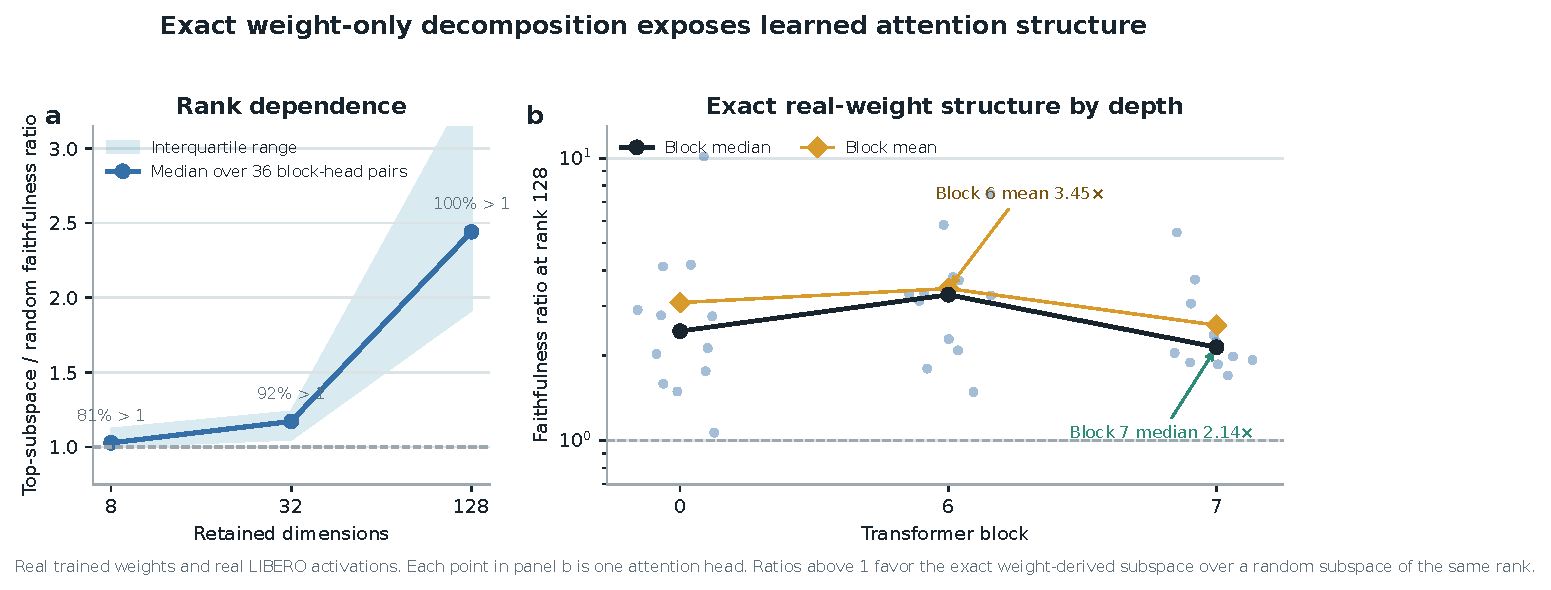
\includegraphics[width=0.94\textwidth]{../paper_figures/main_exact_attention_odt.pdf}
\caption{\textbf{Exact weight-derived attention structure.} Ratios above one favor the exact
weight-derived subspace over a random equal-rank subspace. Each point in the right panel is one
trained attention head.}
\label{fig:exactattention}
\end{figure}

At ranks $8$, $32$, and $128$, respectively, $80.6\%$, $91.7\%$, and $100\%$ of the $36$
block-head pairs favor the exact subspace. Their median ratios are $1.028$, $1.171$, and
$2.441$. At rank $128$, the mean ratio is $3.033$ and the strongest head reaches $10.135$.
The rank-$128$ block means are $3.08$, $3.45$, and $2.56$ for blocks $0$, $6$, and $7$.

This extends exact weight-only construction through individual attention layers. It is not an
exact end-to-end decomposition of the complete policy. Composition across all eight blocks
still faces rapid degree and representation growth.

% ============================================================================
\section{Causal policy structure and a language shortcut}
\label{sec:causal}
% ============================================================================

We next test whether the identified structure affects closed-loop behavior and whether high
task success reflects robust use of the language input.

\subsection{Causal visual subspace}

At the visual bond before the joint backbone, we rank directions separately for translation,
rotation, and gripper actions. We compare the selected subspace with random equal-width
subspaces in offline action reconstruction and closed-loop intervention. This ranking uses
held-out activations and downstream sensitivity. It is causal, but not a weight-only discovery
result.

\begin{figure}[H]
\centering
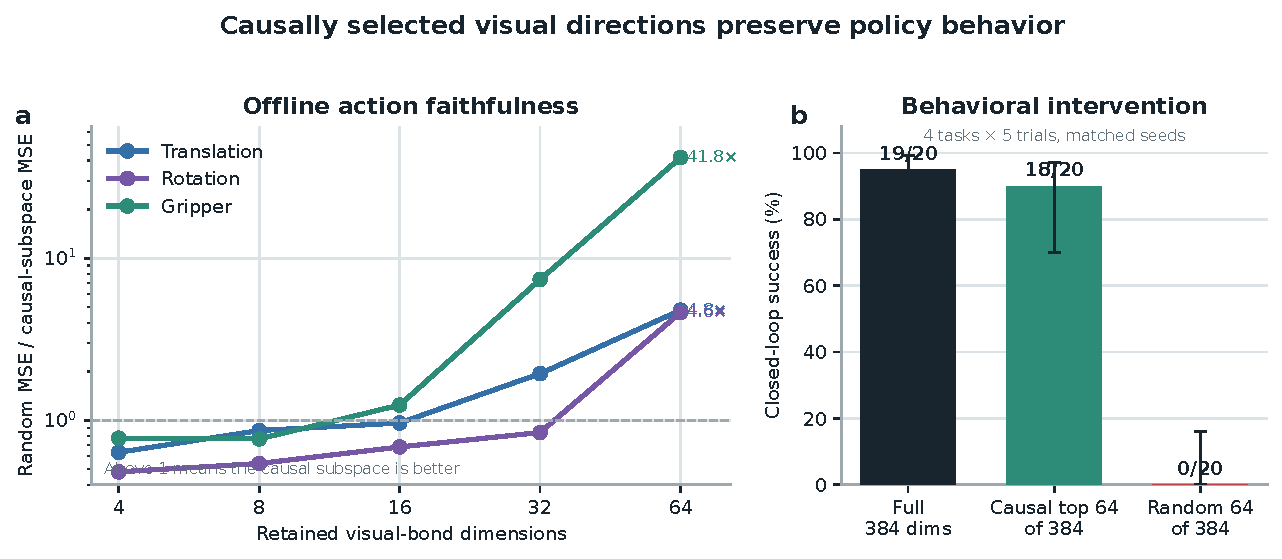
\includegraphics[width=0.94\textwidth]{../paper_figures/main_causal_subspace.pdf}
\caption{\textbf{Causally selected visual directions preserve policy behavior.} The left panel
reports random MSE divided by selected-subspace MSE. The right panel intervenes on the real
policy over four tasks and five paired trials per task.}
\label{fig:causal}
\end{figure}

With $64$ of $384$ dimensions retained, the selected subspace reduces action reconstruction
error relative to random by $4.8\times$ for translation, $4.6\times$ for rotation, and
$41.8\times$ for the gripper. In closed loop, the full representation succeeds in $19/20$
trials, the selected subspace in $18/20$, and a random subspace in $0/20$.

This result establishes a causal low-dimensional substrate, but it is still limited to one
checkpoint and twenty rollouts. The current ranking at this full-policy bond uses held-out
examples and downstream sensitivity. The exact layerwise attention method in
Section~\ref{sec:exactattention} must still be connected to the same full-suite closed-loop
intervention.

\subsection{Counterfactual instruction test}

High success does not guarantee robust language use. We hold the image and robot state fixed
and replace the instruction with one naming another visible object. Across $80$ canonical
one-step trials, the predicted reach direction shifts toward the newly named object in only
$15.0\%$. Mean directional cosine to the named object falls from $0.525$ under the true
instruction to $0.299$ under the counterfactual instruction, while cosine to the original
target remains $0.464$. In an earlier $40$-step closed-loop screen, $33.3\%$ finish closer to
the new object and $55.6\%$ move measurably toward it.

The likely shortcut is structural in the dataset. Each scene template is paired with an almost
fixed target, so scene identity can substitute for object-name grounding. Decorrelated
scripted demonstrations improve the counterfactual metric, but all three fine-tuning attempts
severely reduce ordinary closed-loop success. The best repaired dataset raises capability only
to $21.5\%$, far below the healthy range.

This negative result narrows the VLA claim. The current model is a capable language-conditioned
specialist, but it is not yet a robust instruction-grounded policy. LIBERO-CF independently
documents the same broad failure class in existing VLAs \cite{liberocf}. Our prospective
novelty is therefore not the shortcut alone. It is the harder test of whether exact
weight-derived terms can localize and selectively repair that shortcut.

% ============================================================================
\section{Related work and limitations}
% ============================================================================

\paragraph{Related work.}
OpenVLA and OpenVLA-OFT establish pretrained VLA and continuous-control baselines
\cite{openvla,openvlaoft}. Bilinear MLPs, $\chi$-nets, and bilinear IMPALA policies show that
multiplicative weights can expose low-rank structure and causal controls
\cite{pearce,chinets,bimpala}. Recent work also steers pretrained VLAs through activation
directions \cite{haonsteering}. Our distinction is the exact weight-derived construction in a
policy designed as a rational tensor program. Tensor and polynomial networks provide the broader
multilinear foundation \cite{koldabader,stoudenmire,chrysos}. VLA robustness benchmarks show
that standard LIBERO success can coexist with weak language use
\cite{liberopro,liberocf,liberopara}.

\paragraph{Limitations and conclusion.}
No same-skeleton conventional twin yet measures conversion cost. The benchmark is one specialist
suite, the policy fails a counterfactual instruction test, and exact decomposition is layerwise
rather than end to end. The closed-loop subspace test uses one checkpoint and twenty trials, while
the first direct coefficient edit fails its selectivity gate. The defensible result is therefore
narrow: rational restrictions do not prevent competitive LIBERO-Object control, and they provide
a precise weight-derived analysis surface. Broader grounding, matched controls, and validated
coefficient edits remain necessary.

\paragraph{Reproducibility.}
The final artifact will provide code, configurations, checkpoint hashes, exact certificates, and
per-episode logs. Canonical-state checks fail loudly when requested states are unavailable.

% ============================================================================
\clearpage
\begin{thebibliography}{99}

\bibitem{openvla}
M.~J. Kim et al.
\newblock \emph{OpenVLA: An Open-Source Vision-Language-Action Model.}
\newblock CoRL, 2024.

\bibitem{openvlaoft}
M.~J. Kim, C.~Finn, and P.~Liang.
\newblock \emph{Fine-Tuning Vision-Language-Action Models: Optimizing Speed and Success.}
\newblock 2025.

\bibitem{pearce}
A.~Rigg, T.~Dooms, M.~T. Pearce, J.~Oramas, and L.~Sharkey.
\newblock \emph{Bilinear MLPs Enable Weight-Based Mechanistic Interpretability.}
\newblock ICLR, 2025.

\bibitem{chinets}
T.~Dooms, W.~Gauderis, G.~A. Wiggins, and J.~Oramas.
\newblock \emph{Compositionality Unlocks Deep Interpretable Models.}
\newblock 2025.

\bibitem{bimpala}
F.~Oozeer, Y.~Erisken, A.~Rigg, J.~Oramas, and L.~Sharkey.
\newblock \emph{Bilinear Convolution Decomposition for Causal RL Interpretability.}
\newblock 2024.

\bibitem{haonsteering}
B.~H\"aon, K.~Stocking, I.~Chuang, and C.~Tomlin.
\newblock \emph{Mechanistic Interpretability for Steering Vision-Language-Action Models.}
\newblock 2025.

\bibitem{sparsecircuits}
S.~Marks et al.
\newblock \emph{Sparse Feature Circuits: Discovering and Editing Interpretable Causal Graphs
in Language Models.}
\newblock ICLR, 2025.

\bibitem{causalreduction}
M.~Keki\'c et al.
\newblock \emph{Learning Nonlinear Causal Reductions to Explain Reinforcement Learning
Policies.}
\newblock ICLR, 2026.

\bibitem{liberopro}
X.~Zhou et al.
\newblock \emph{LIBERO-PRO: Towards Robust and Fair Evaluation of Vision-Language-Action
Models Beyond Memorization.}
\newblock 2025.

\bibitem{liberocf}
Y.~Fang et al.
\newblock \emph{When Vision Overrides Language: Evaluating and Mitigating Counterfactual
Failures in VLAs.}
\newblock 2026.

\bibitem{liberopara}
C.~Kim et al.
\newblock \emph{LIBERO-Para: A Diagnostic Benchmark and Metrics for Paraphrase Robustness in
VLA Models.}
\newblock 2026.

\bibitem{koldabader}
T.~Kolda and B.~Bader.
\newblock \emph{Tensor Decompositions and Applications.}
\newblock SIAM Review, 2009.

\bibitem{stoudenmire}
E.~Stoudenmire and D.~Schwab.
\newblock \emph{Supervised Learning with Tensor Networks.}
\newblock NeurIPS, 2016.

\bibitem{chrysos}
G.~Chrysos et al.
\newblock \emph{Deep Polynomial Neural Networks.}
\newblock CVPR and TPAMI, 2020 to 2021.

\end{thebibliography}

% ============================================================================
\appendix
\section{Supporting results and decisions}
% ============================================================================

\subsection{Original 94.5\% capability result}

Before the final protocol-aligned benchmark, one rational ViT checkpoint succeeded in
$189/200$ trials under a $600$-step horizon and $20$ trials per task. This result established
that the rational implementation could support all ten tasks. It should not be compared
directly with the protocol-aligned external references because it uses one training seed, fewer
trials, and a longer horizon.

\subsection{Per-task ensemble behavior}

\begin{figure}[H]
\centering
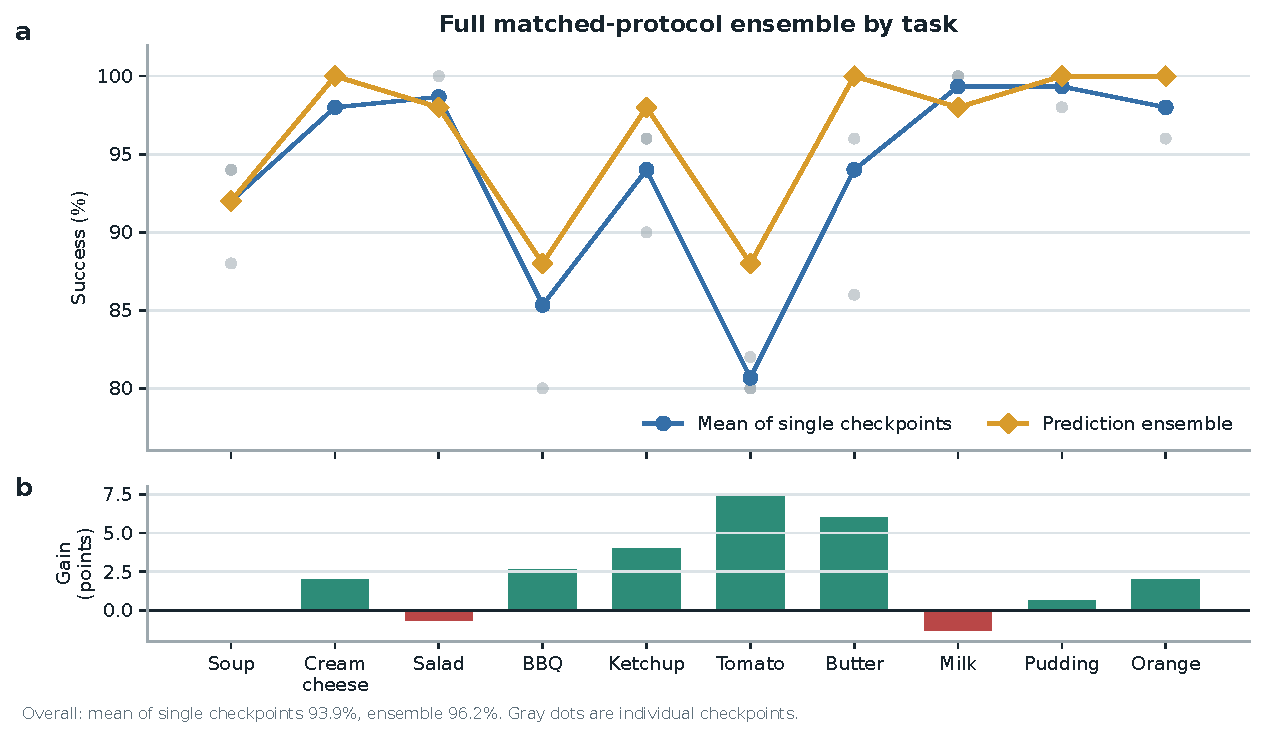
\includegraphics[width=0.96\textwidth]{../paper_figures/appendix_ensemble_per_task.pdf}
\caption{\textbf{Per-task effect of prediction averaging.} Gray points are the three
convolutional checkpoints, evaluated with $50$ canonical trials per task. Curves compare their
taskwise mean with elementwise action-prediction averaging. The ensemble raises overall success
from a $93.9\%$ member mean to $96.2\%$, with its largest gains on tomato sauce, butter, and
ketchup. It requires three forward passes and is not a single $20.1$M-parameter policy.}
\label{fig:ensemble-task}
\end{figure}

\subsection{Product-routing multimodal head}

For an action-query state $h$, the product-routing head represents
\begin{equation}
a(h,b)=c_0(h)+\sum_{g=1}^{G}(2b_g-1)c_g(h),
\qquad b\in\{0,1\}^{G}.
\end{equation}
The center, offsets, and gates are bilinear CP modules. A final external sign choice selects
one of $2^G$ modes. The head folds to numerical precision, but its five-seed closed-loop mean
is $44\%\pm30\%$ and its range overlaps the linear baseline. The strongest rational policy
therefore uses the linear head. Product routing remains a construction result until it wins a
controlled genuinely multimodal task.

\subsection{Development interventions}

Focused DAgger on BBQ and tomato improves combined success from $82.5\%$ to $96.0\%$ using
seven corrective episodes and $1{,}131$ frames. Applying the same update thinly across all ten
tasks reduces overall success from $92.0\%$ to $72.0\%$. Three original AWR runs decline by
$8.0$, $4.6$, and $2.6$ points. A reward audit shows that accumulated step cost makes every
successful trajectory have negative return. After removing that term and repairing the
terminal boundary, one pilot improves by two points. These are development diagnostics, not
validated paper contributions.

\begin{figure}[H]
\centering
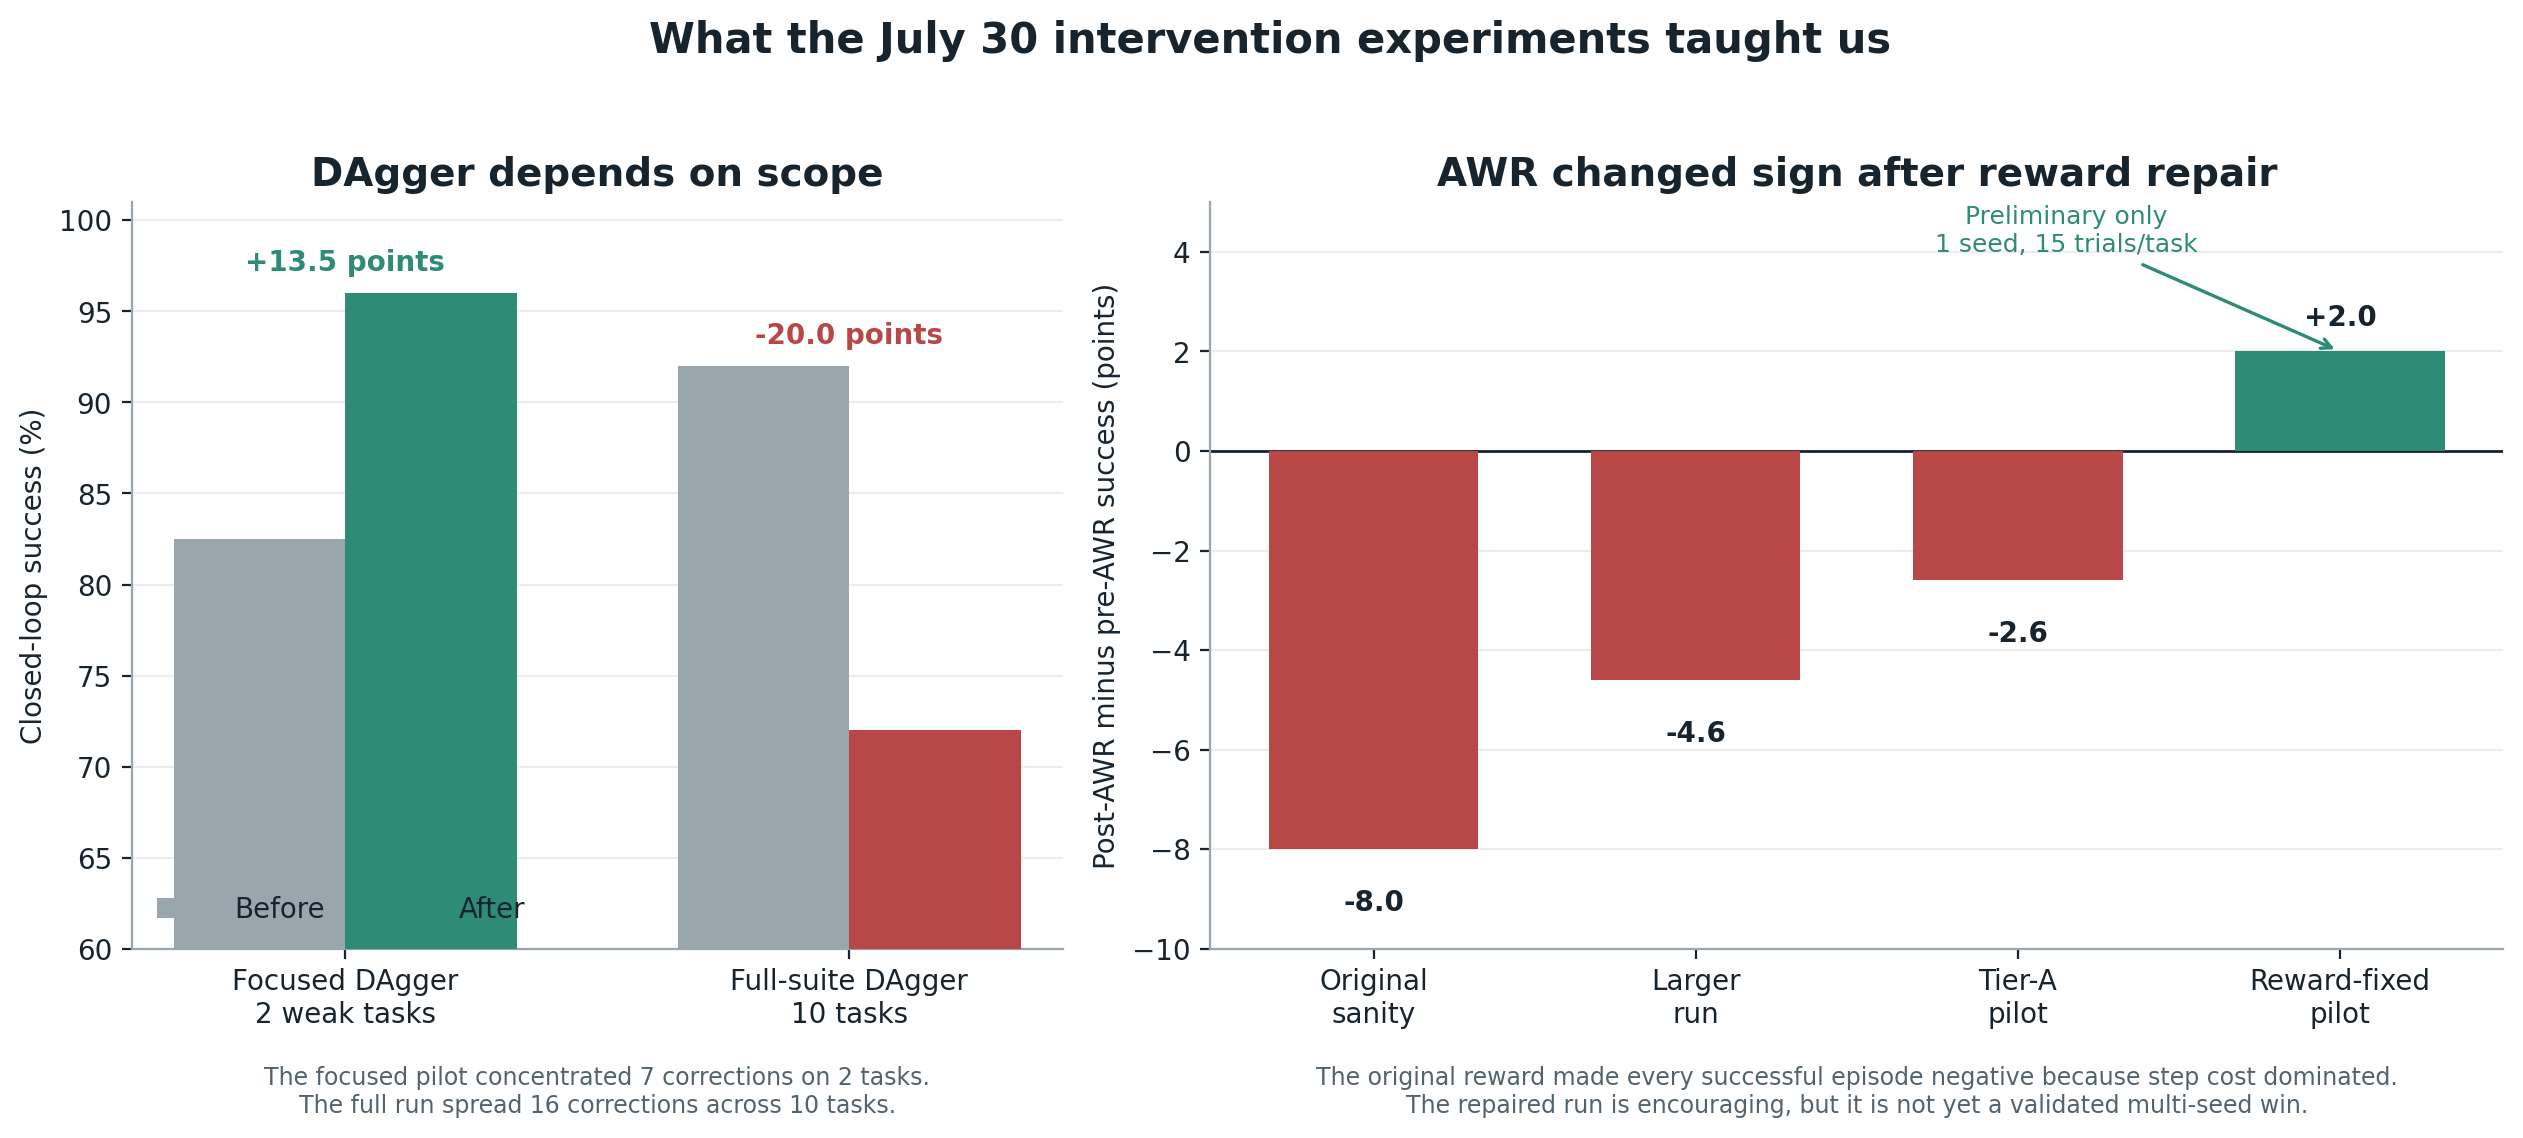
\includegraphics[width=0.98\textwidth]{../progress_figures/intervention_results.png}
\caption{\textbf{Development interventions reveal scope and reward sensitivity.} Focused
DAgger helps two weak tasks, while spreading a small correction budget across ten tasks causes
regression. Three AWR variants also regress before a reward audit and repair. The positive
reward-repaired AWR result is a one-seed pilot with $15$ trials per task, so it is not evidence
of a validated improvement.}
\label{fig:development-interventions}
\end{figure}

\subsection{Expanded attention screen and first direct edit}
\label{app:expanded-mechanisms}

The corrected fixed-control attention analysis covers all eight blocks and twelve heads. At
rank $128$, $83/96$ block-head pairs favor the exact weight-derived subspace. The median ratio
is $1.94$, the mean is $2.58$, and blocks $2$ and $3$ provide useful weak or negative controls.
At ranks $8$ and $32$, only $54/96$ and $60/96$ pairs favor the exact subspace. The effect is
therefore depth-dependent and strongest at the wider tested rank.

The first direct weight-edit screen uses four tasks and five paired canonical episodes per
task. Exact-subspace retention preserves $18/20$ successes compared with $16/20$ for both
random controls. This $10$-point advantage misses the preregistered $15$-point gate. Exact
removal also preserves $18/20$, compared with $17/20$ for both random controls, which is the
wrong direction for the necessity prediction. The screen is a no-go for the current mapping
from Gram eigenspaces to query, key, and value column edits.

\begin{figure}[H]
\centering
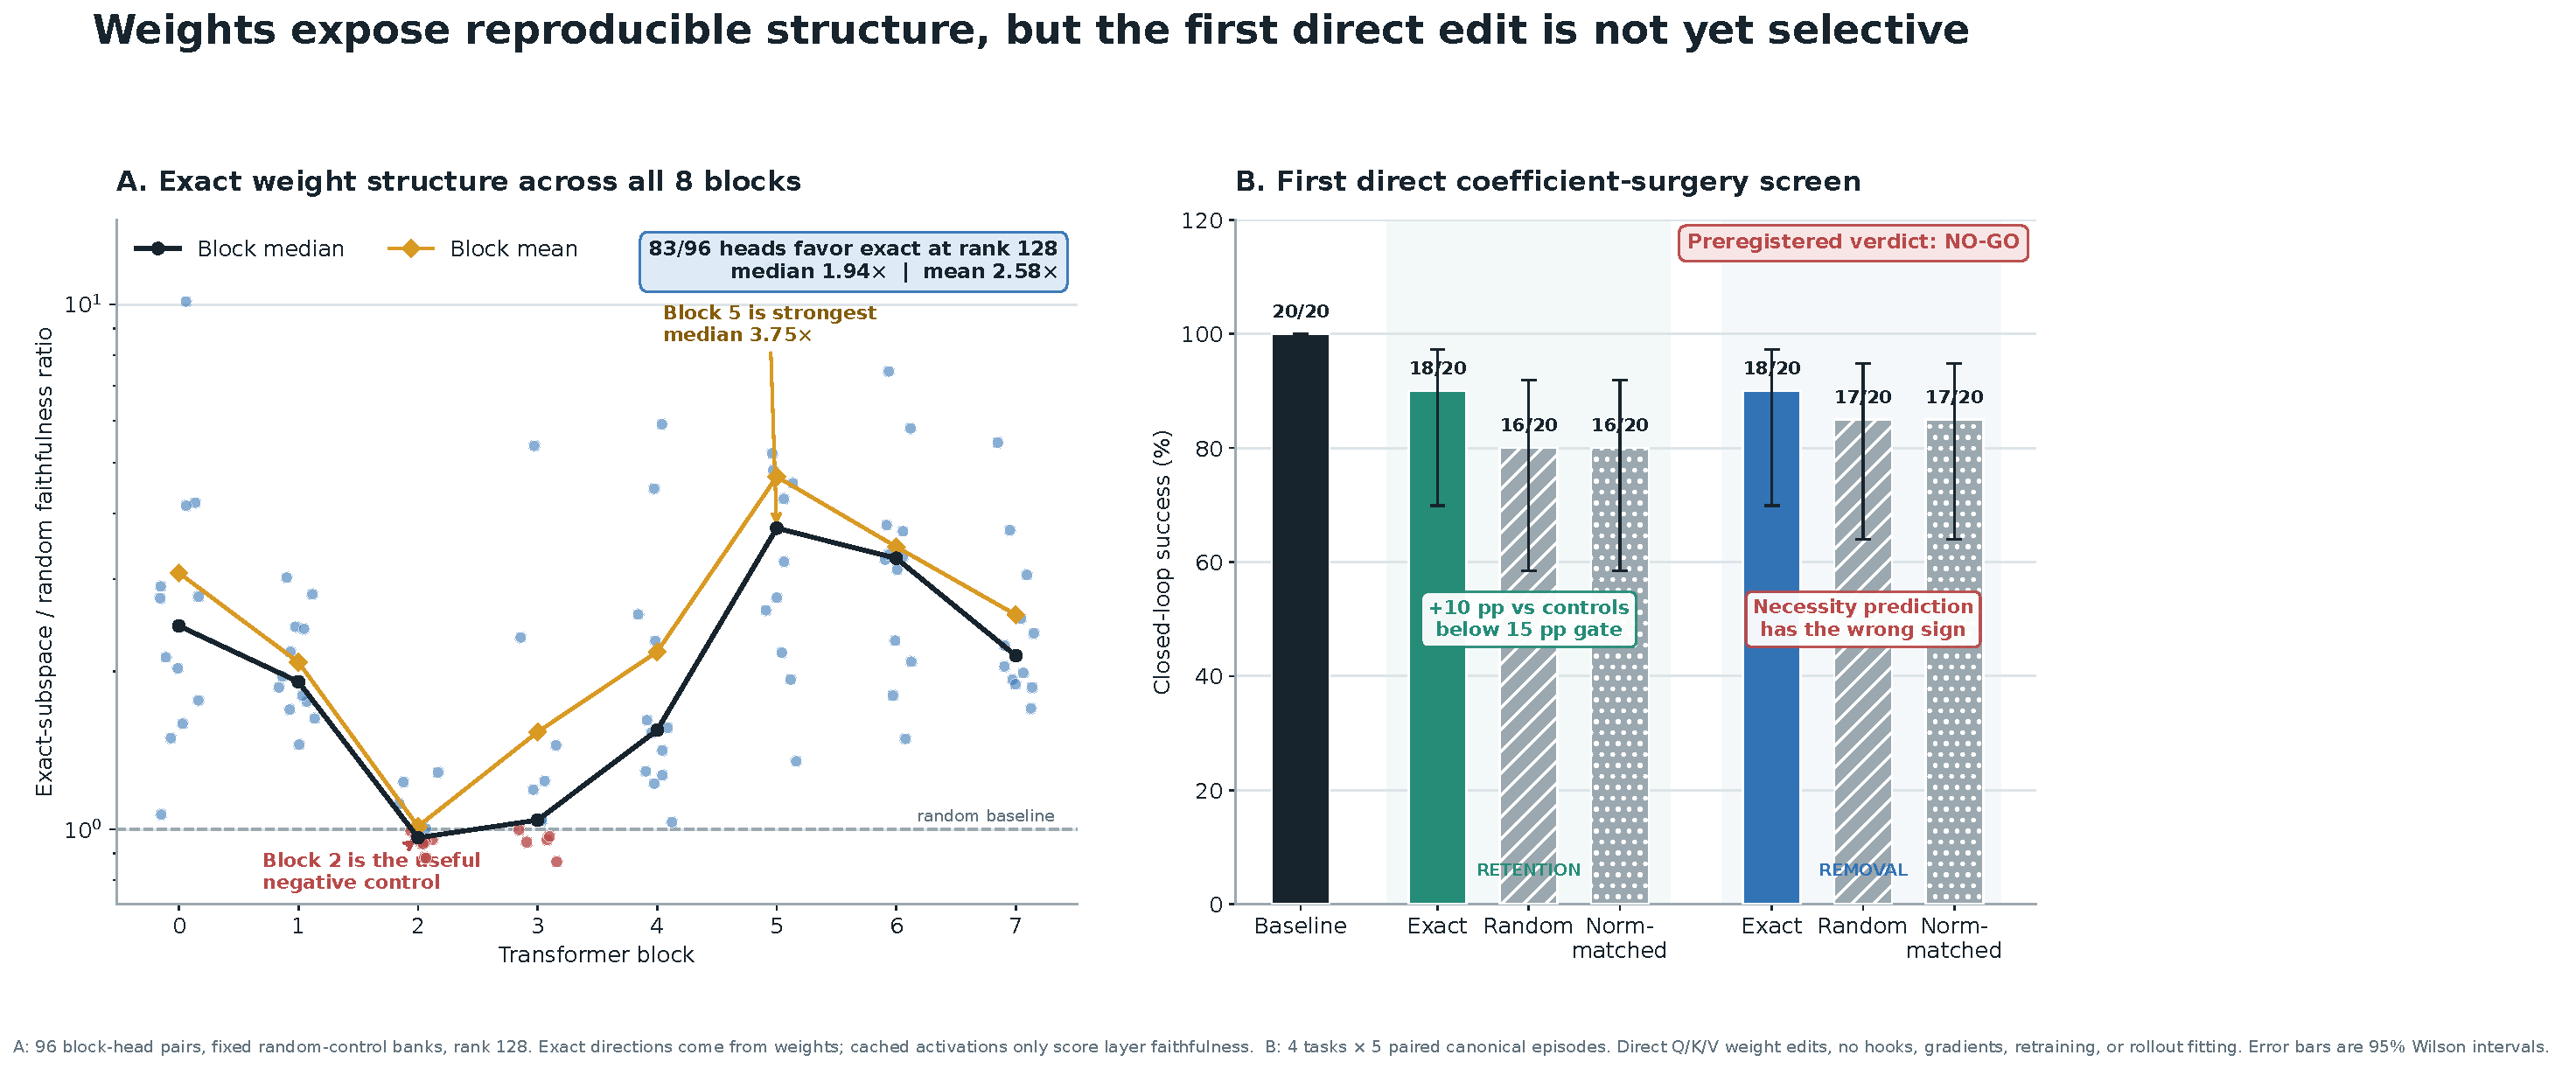
\includegraphics[width=0.98\textwidth]{../paper_figures/presentation_july31_mechanism_results.pdf}
\caption{\textbf{Expanded weight-structure and direct-surgery results.} Left: all $96$
block-head pairs at rank $128$, with fixed random-control banks. Exact directions come from
weights, while cached activations only score layer faithfulness. Right: the first direct
query-key-value column-edit screen over four tasks and five paired trials per task. Error bars
are $95\%$ Wilson intervals. The preregistered verdict is no-go because retention misses the
effect-size gate and removal has the wrong sign.}
\label{fig:expanded-mechanisms}
\end{figure}

\subsection{Numerical scope of rational conversion}

The deployed Pad\'e computation is exactly rational even though it approximates RMS
normalization. Final certification must report its polynomial degrees, coefficients,
denominator margin, observed activation range, tail error, action drift, and runtime overhead.
Operator membership alone does not establish practical numerical safety under distribution
shift.

\end{document}
